The model we investigate here is of $L$ unlinked loci at which mutations affect
the trait. These mutations are randomly assigned values from a distribution of
mutational effect sizes and these effects act additively both within and between
loci. The resulting trait values in haploid individuals are the sum of all
mutations occurring in their history, and correlations between individuals arise
because mutations fall on shared portions of genealogies at individual loci.
Because the loci are unlinked we assume their genealogies are independent. This
model is shown schematically in Figure \ref{fig:schema}.

The genealogy at a locus is represented by the random vector of branch lengths,
$\mathbf{T}$. An element $T_{\omega}$ of $\mathbf{T}$ is the branch length
subtending only individuals in the set $\omega$ and no others in the sample. For
example, $T_{\{a,b\}}$ is the length of the branch subtending only individuals
$a$ and $b$. If such a branch does not exist for a given genealogy the branch
length is set to zero. In this way $\mathbf{T}$ encodes both the branch lengths
and topology of a genealogy. $\Omega$ is the set of all possible branches. If
there are three sampled individuals, $a$, $b$, and $c$, then
$\Omega=\{\{a\},\{b\},\{c\},\{a,b\},\{a,c\},\{b,c\}\}$ and
$\mathbf{T}=(T_{\{a\}},T_{\{b\}},T_{\{c\}},T_{\{a,b\}},T_{\{a,c\}},T_{\{b,c\}})$.
Realizations of the branch lengths are denoted using the same notation with
lowercase letters. The moment generating functions for the distribution of
branch lengths is $\varphi_{\mathbf{T}}$. 

Within each locus an infinite number of mutation are possible and the mutation
rate per unit of coalescent time to mutations affecting the trait is $\T$. That
is, $\T$ is the mutation rate for the entire locus. Each mutation affecting the
trait is assigned an effect size from a probability distribution of effect
sizes. The mgf of this distribution is written as $\psi()$ and the $i^{th}$
(non-central) moment is $m_i$. Mutational effects behave additively both within
and between loci.

The principle random quantities resulting from this process are the quantitative
trait values which we will hereafter refer to these as trait values. Starting
with a trait controlled by a single locus, the random vector of trait values in
the sampled individuals is $\mathbf{Y}$, such that for sampled individuals $a$,
$b$, and $c$, $\mathbf{Y}=\{Y_a,Y_b,Y_c\}$. The trait values are modeled as the
change relative to the value in the most recent common ancestor of the sample at
that locus. Since we do not know what the ancestral value was, this cannot be
directly observed. For a trait controlled by multiple loci, $\mathbf{Y}$ is the
sum over contributions from these loci, each measured with respect to an
arbitrary value. However, $\mathbf{Y}$ is sufficient to determine measurable
quantities like differences in trait values between individuals or a sample
variance. The moment generating functions for the distribution of branch lengths
is $\varphi_{\mathbf{Y}}$.

\begin{figure}
  \centering
  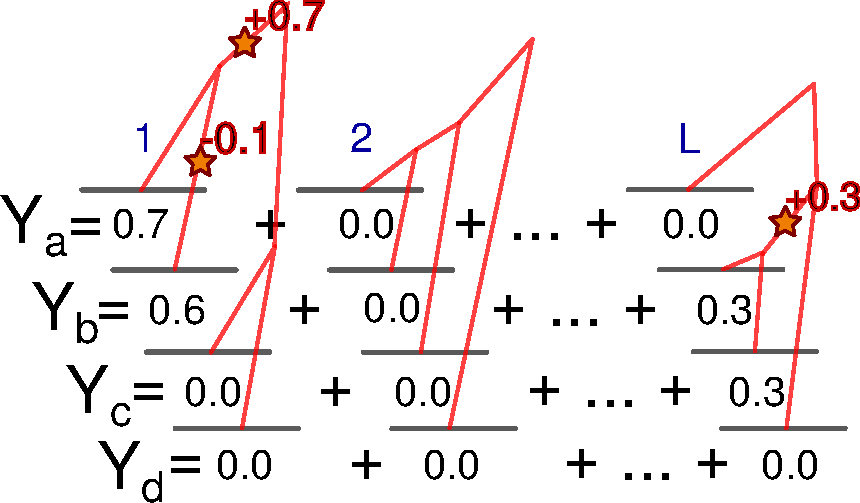
\includegraphics[width=0.8\textwidth]{figures/schema.pdf}
  \caption{A schematic representation of the model analyzed.
  $L$ loci affect the trait in a set of individuals and have independent
  genealogies. Mutations occur within loci as a Poisson process and act
  additively to give individual trait values. Potentially many loci affecting
  the trait may receive no mutations.}
  \label{fig:schema}
\end{figure}

When we refer to the genetic architecture of a trait this is used to mean the
combination of genetic parameters affecting the trait distribution ($L$, $\T$,
$\psi()$). The realized distribution for a given genetic architecture is
therefore a random quantity. Another useful way to describe a trait is by its
sparsity. The sparsity of a trait refers to how many segregating mutations
affect it. A more `sparse' trait is affected by fewer mutations. We formally
measure this as the average number of pairwise differences separating two
randomly chosen haplotypes at loci affecting the trait. Sparsity thus depends
both on the genetic architecture through the mutation rate and the distribution
of coalescence times.

At various points additional genealogical quantities are helpful when presenting
results. For populations of exchangeable individuals an important summary of the
distribution of genealogies is $\mathbbm{T}_{i,j}$ which gives the amount of
time that $i$ lineages remain from a sample of size $j$. It also useful to have
a symbol for the pairwise coalescent time between a linage in individual $i$ and
in individual $j$. Here, we write this as $\mathcal{T}_{i,j}$. When considering
structured populations $\mathcal{T}_{a,b}$ gives the coalescence time between a
lineage from subpopulation $a$ and a lineage from subpopulation $b$. A final set
of quantities are defined for sums of branch lengths. Let $\tau_{a+b}$ be the
sum of all branches containing both $a$ and $b$, and $\tau_{a/b}$ be the sum of
all branches containing $a$ and not $b$. Extensions of this for more than two
individuals are also used. The same notation is used when referring to sets of
branch indices. So $\Omega_{a+b}$ and $\Omega_{a/b}$ would be the sets of
branches summed to give $\tau_{a+b}$ and $\tau_{a/b}$ respectively.


%% It is useful to first describe various quantities of interest and their
%% notation. A first set of parameters define what we will refer to as the genetic
%% architecture of the trait. $L$ gives the number of loci at which mutations
%% affect the trait, and $\T$ gives the mutation rate. The other important
%% component of the genetic architecture is the distribution of effect sizes of
%% mutations. The mgf of this distribution is written as $\psi()$ and the $i^{th}$
%% (non-central) moment of this distribution is $m_i$. The sparsity of a trait
%% refers to how many segregating mutations affect it. We formally measure this as
%% the average number of pairwise differences separating two randomly chosen
%% haplotypes at loci affecting the trait. Sparsity thus depends both on the
%% genetic architecture through the mutation rate and the distribution of
%% coalescence times.


%% The random vector of branch lengths describing the genealogy at a locus is
%% $\mathbf{T}$, and an element $T_{a,b}$ of $\mathbf{T}$ is the branch length
%% subtending individuals $a$ and $b$. $\omega$ will be used to denote a particular
%% set of individuals and hence a branch on the genealogy such that $T_\omega$ is
%% then length of branch $\omega$. $\Omega$ is the set of all possible branches.
%% For instance, if there are three sampled individuals, $a$, $b$, and $c$, then
%% $\mathbf{Y}=\{Y_a,Y_b,Y_c\}$,
%% $\mathbf{T}=\{T_a,T_b,T_c,T_{a,b},T_{a,c},T_{b,c}\}$, and
%% $\Omega=\{(a),(b),(c),(a,b),(a,c),(b,c)\}$. Realizations of the random trait
%% values and branch lengths are denoted using the same notation with lowercase
%% letters. The moment generating functions for the distribution of branch lengths
%% and distribution of trait values are $\varphi_{\mathbf{T}}$ and
%% $\varphi_{\mathbf{Y}}$.

%% For populations of exchangeable individuals an important summary of the
%% distribution of genealogies is $T_{i,j}$ which gives the amount of time that $i$
%% lineages remain from a sample of size $j$. In structured populations an equally
%% important quantity is $\tau_{i,j}$ which gives the coalescence time between a
%% lineage from subpopulation $i$ and a lineage from subpopulation $j$.

%% A final piece of notation is for sums of branch lengths. Let $\tau_{a+b}$ be the
%% (random) sum of all branches containing both $a$ and $b$. Conversely,
%% $\tau_{a/b}$ will be the random sum of all branches containing $a$ and not $b$.
%% Extensions of this for more than two individuals are also used. The same
%% notation is used when referring to sets of branch indices. So $\Omega_{a+b}$ and
%% $\Omega_{a/b}$ would be the sets of branches summed to give $\tau_{a+b}$ and
%% $\tau_{a/b}$.

%%% Local Variables:
%%% TeX-master: "short_report.tex"
%%% End:
